% 导言区
\documentclass{ctexart}

%\usepackage{ctex}       % 中文处理宏包
\usepackage{graphicx}
\graphicspath{{figures/}}   % 图片在当前目录下的figures目录

% 标题控制(caption、bicaption等宏包)
% 并排与子图表(subcaption、subfig、floatrow等宏包)
% 绕排(picinpar、wrapfig等宏包)

% 浮动体
% 实现灵活分页(避免无法分割的内容产生的页面留白)
% 给图表添加标题
% 交叉引用

% Figure环境(table环境与之类似)
% \begin{figure}[<允许位置>]
%   <任意内容>
% \end{figure}

% <允许位置>参数(默认tbp)
% h,此处(here)-代码所在的上下文位置
% t,页顶(top)-代码所在页面或之后页面的顶部
% b,页底(bottom)-代码所在页面或之后页面的底部
% p,独立一页(page)-浮动页面


% 正文区
\begin{document}
    \LaTeX{} 中系统的吉祥物---小狮子见图 \ref{fig-lion}
    \begin{figure}[h]
        \centering
        
\includegraphics[scale=0.3]{lion.jpg}
        \caption{\LaTeX 系统的吉祥物---小狮子} \label{fig-lion}
    \end{figure}

    遥望太白,看积雪能皑,别有一番风景(图\ref{fig-mountain})。
    \begin{figure}[h]
        \centering
        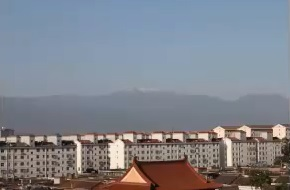
\includegraphics[scale=0.5]{mountain.jpg}
        \caption{太白山} \label{fig-mountain}
    \end{figure}

    熟练使用 \LaTeX 中的Tikz,可以绘制如图 \ref{fig-parallelepiped} 所示的精美矢量图。
    \begin{figure}[htbp]
        \centering
        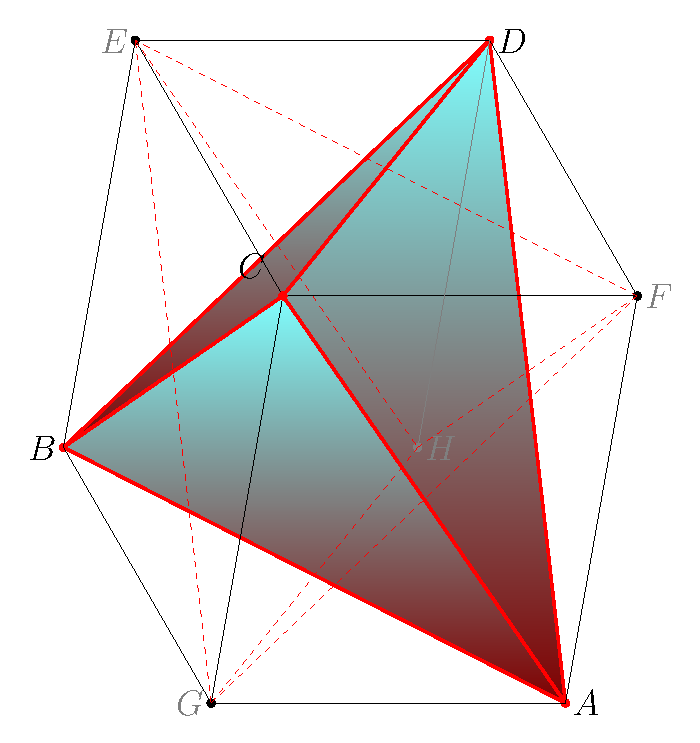
\includegraphics[scale=0.2]{parallelepiped.pdf}
        \caption{parallelepiped} \label{fig-parallelepiped}
    \end{figure}

    \LaTeX{} 中的表格 \ref{tab-score}:
    \begin{table}[htbp]
        \centering
        \caption{考试成绩单} \label{tab-score}
        \begin{tabular}{|l||c|c|r|r|}
            \hline
            姓名 & 语文 & 数学 & 外语 & 备注 \\
            \hline \hline
            张三 & 87 & 100 & 93 & 优秀 \\
            \hline
            李四 & 75 & 64 & 52 & 补考另行通知 \\
            \hline
            王二 & 80 & 82 & 78 & \\
            \hline
        \end{tabular}
    \end{table}
    
\end{document}